\chapter{Existing Environments}

A lot of multi agent systems have already been developed, and we will take a look at a few of them, to get an idea of how others have designed multi agent systems.\\
\\
\section{Net-Logo}
NetLogo is a popular and widespread environment for programming in a MAS language, developed by a man called Uri Wilensky in '99, who is currently working at the Northwestern University \cite{misc:northwestern}.\\ \indent NetLogo features a very easy programming language for both creating Agents and defining Environments, and also provides relatively easy ways of manipulating the cosmetics of the MAS-simulation. NetLogo has the advantages that even though the programming language is very easy to learn and use, it is also very feature rich, and can create MAS's that can simulate almost any possible scenario, right from advanced traffic scenarios to how many tadpoles will survive the first week of their lives. \\
\\
The code, shown in the following code-snippet, will generate a simple test with color-mixing, to simulate passing of genes.

\begin{NetLogo}{This is a NetLogo sorce code example}{}
to setup
  clear-all
  ask patches
    [ set pcolor (random colors) * 10 + 5
        if pcolor = 75  ;; 75 is too close to another color so change it to 125
          [ set pcolor 125 ] ]
  reset-ticks
end

to go
  ask patches [ set pcolor [pcolor] of one-of patches ]
  tick
end


; Copyright 1997 Uri Wilensky. All rights reserved.
; The full copyright notice is in the Information tab.
\end{NetLogo}

This very small code example will, together with the NetLogo GUI, create the elaborate simulation shown in \ref{fig:NetLogoscreen}. All of this simulation data is saved in NetLogos custom file format, so that they can easily be run by someone else.

\begin{figure}[H]
\begin{center}
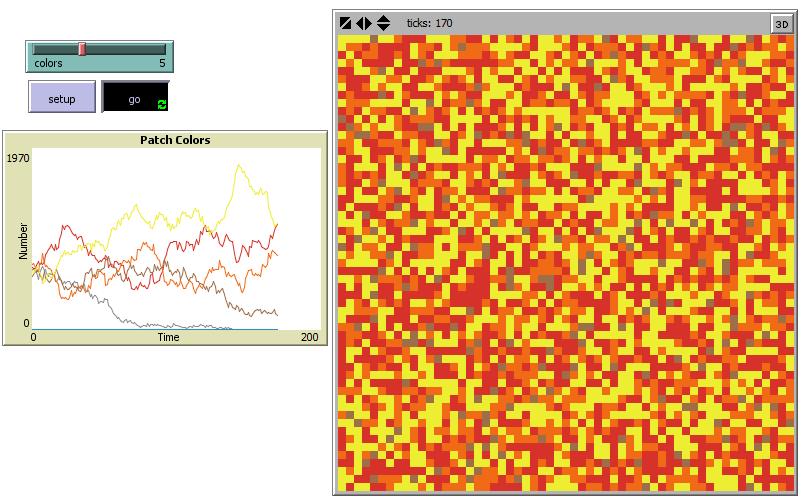
\includegraphics[width=\textwidth*0.9]{Images/NetLogo.png}%
\end{center}
\caption{Simple Netlogo Simulation}%
\label{fig:NetLogoscreen}%
\end{figure}

%One example of a MAS is the NetLogo application \cite{misc:netlogo}.\\